% Options for packages loaded elsewhere
\PassOptionsToPackage{unicode}{hyperref}
\PassOptionsToPackage{hyphens}{url}
%
\documentclass[
]{book}
\usepackage{amsmath,amssymb}
\usepackage{lmodern}
\usepackage{iftex}
\ifPDFTeX
  \usepackage[T1]{fontenc}
  \usepackage[utf8]{inputenc}
  \usepackage{textcomp} % provide euro and other symbols
\else % if luatex or xetex
  \usepackage{unicode-math}
  \defaultfontfeatures{Scale=MatchLowercase}
  \defaultfontfeatures[\rmfamily]{Ligatures=TeX,Scale=1}
\fi
% Use upquote if available, for straight quotes in verbatim environments
\IfFileExists{upquote.sty}{\usepackage{upquote}}{}
\IfFileExists{microtype.sty}{% use microtype if available
  \usepackage[]{microtype}
  \UseMicrotypeSet[protrusion]{basicmath} % disable protrusion for tt fonts
}{}
\makeatletter
\@ifundefined{KOMAClassName}{% if non-KOMA class
  \IfFileExists{parskip.sty}{%
    \usepackage{parskip}
  }{% else
    \setlength{\parindent}{0pt}
    \setlength{\parskip}{6pt plus 2pt minus 1pt}}
}{% if KOMA class
  \KOMAoptions{parskip=half}}
\makeatother
\usepackage{xcolor}
\usepackage{longtable,booktabs,array}
\usepackage{calc} % for calculating minipage widths
% Correct order of tables after \paragraph or \subparagraph
\usepackage{etoolbox}
\makeatletter
\patchcmd\longtable{\par}{\if@noskipsec\mbox{}\fi\par}{}{}
\makeatother
% Allow footnotes in longtable head/foot
\IfFileExists{footnotehyper.sty}{\usepackage{footnotehyper}}{\usepackage{footnote}}
\makesavenoteenv{longtable}
\usepackage{graphicx}
\makeatletter
\def\maxwidth{\ifdim\Gin@nat@width>\linewidth\linewidth\else\Gin@nat@width\fi}
\def\maxheight{\ifdim\Gin@nat@height>\textheight\textheight\else\Gin@nat@height\fi}
\makeatother
% Scale images if necessary, so that they will not overflow the page
% margins by default, and it is still possible to overwrite the defaults
% using explicit options in \includegraphics[width, height, ...]{}
\setkeys{Gin}{width=\maxwidth,height=\maxheight,keepaspectratio}
% Set default figure placement to htbp
\makeatletter
\def\fps@figure{htbp}
\makeatother
\setlength{\emergencystretch}{3em} % prevent overfull lines
\providecommand{\tightlist}{%
  \setlength{\itemsep}{0pt}\setlength{\parskip}{0pt}}
\setcounter{secnumdepth}{5}
\ifLuaTeX
\usepackage[bidi=basic]{babel}
\else
\usepackage[bidi=default]{babel}
\fi
\babelprovide[main,import]{brazilian}
% get rid of language-specific shorthands (see #6817):
\let\LanguageShortHands\languageshorthands
\def\languageshorthands#1{}
\usepackage{booktabs}
\ifLuaTeX
  \usepackage{selnolig}  % disable illegal ligatures
\fi
\usepackage[]{natbib}
\bibliographystyle{plainnat}
\IfFileExists{bookmark.sty}{\usepackage{bookmark}}{\usepackage{hyperref}}
\IfFileExists{xurl.sty}{\usepackage{xurl}}{} % add URL line breaks if available
\urlstyle{same} % disable monospaced font for URLs
\hypersetup{
  pdftitle={Bookdown Vídeos, Filmes e Documentários},
  pdfauthor={Daniel Claudino},
  pdflang={pt-BR},
  hidelinks,
  pdfcreator={LaTeX via pandoc}}

\title{Bookdown Vídeos, Filmes e Documentários}
\author{Daniel Claudino}
\date{2022-11-01}

\begin{document}
\maketitle

{
\setcounter{tocdepth}{1}
\tableofcontents
}
\hypertarget{apresentauxe7uxe3o}{%
\chapter{Apresentação}\label{apresentauxe7uxe3o}}

Bookdown Vídeos, Filmes e Documentários

\begin{figure}

{\centering 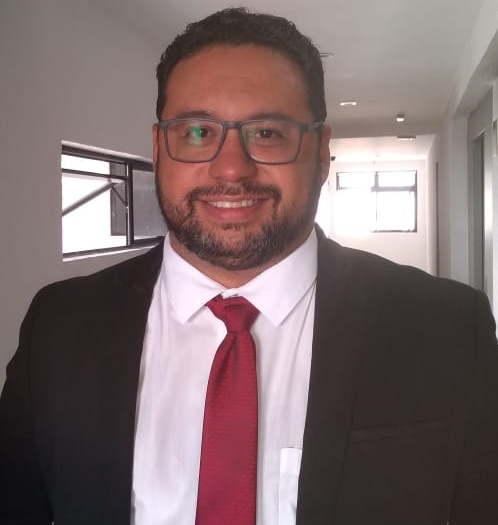
\includegraphics[width=0.5\linewidth]{imagens/FOTO-PERFIL-DANIEL-CLAUDINO-2020} 

}

\caption{-}\label{fig:unnamed-chunk-1}
\end{figure}

Neste bookdown, estarão contidos todos os vídeos, filmes e documentários de todas as disciplinas do 1º ao 10º período. Cada disciplina será tratada como um capítulo.

\hypertarget{controle-de-versuxe3o}{%
\section{Controle de Versão}\label{controle-de-versuxe3o}}

\begin{longtable}[]{@{}
  >{\raggedright\arraybackslash}p{(\columnwidth - 6\tabcolsep) * \real{0.2500}}
  >{\raggedright\arraybackslash}p{(\columnwidth - 6\tabcolsep) * \real{0.2500}}
  >{\raggedright\arraybackslash}p{(\columnwidth - 6\tabcolsep) * \real{0.2500}}
  >{\raggedright\arraybackslash}p{(\columnwidth - 6\tabcolsep) * \real{0.2500}}@{}}
\toprule()
\begin{minipage}[b]{\linewidth}\raggedright
Versão
\end{minipage} & \begin{minipage}[b]{\linewidth}\raggedright
Data / Hora
\end{minipage} & \begin{minipage}[b]{\linewidth}\raggedright
Colaborador
\end{minipage} & \begin{minipage}[b]{\linewidth}\raggedright
Descrição da Contribuição
\end{minipage} \\
\midrule()
\endhead
0.1 & 29/11/2022 12h17 & \href{https://wa.me/5583988853815}{Daniel Claudino} & Versão inicial do bookdown Vídeos, Filmes e Documentários. \\
\bottomrule()
\end{longtable}

\hypertarget{observauxe7uxe3o-importante}{%
\section{Observação Importante}\label{observauxe7uxe3o-importante}}

\textbf{NOTA}: Este material tem como finalidade auxiliar a fixação de assuntos estudados em sala de aula de acordo com os \textbf{planos de ensino das disciplinas}.

Ele \textbf{não deve ser} utilizado como \textbf{único material de estudo para a prova}, então:

\begin{enumerate}
\def\labelenumi{\arabic{enumi}.}
\tightlist
\item
  Consulte os \textbf{slides da professora} na plataforma FTM;\\
\item
  Faça \textbf{notas de aula} do que for tratado em sala de aula;\\
\item
  \textbf{Em caso de dúvidas}: Elas devem ser encaminhadas no grupo de whatsapp da turma.
\end{enumerate}

\hypertarget{p1---anatomia-humana}{%
\chapter{P1 - Anatomia Humana}\label{p1---anatomia-humana}}

Neste capítulo, estarão contidos os vídeos, filmes e documentários da disciplina Anatomia Humana.

\begin{longtable}[]{@{}ll@{}}
\toprule()
Data & Tópicos Abordados \\
\midrule()
\endhead
30/10/2022 & - Versão inicial do documento \\
\bottomrule()
\end{longtable}

\hypertarget{vuxeddeos}{%
\section{Vídeos}\label{vuxeddeos}}

TODOS os Vídeos postados no Grupo de Anatomia do Whatsapp para as provas práticas estão disponíveis em: \url{https://1drv.ms/u/s!Au-CrfNP6c0bha15wnMffwLPUbuLJQ?e=88YJL1}

\begin{itemize}
\tightlist
\item
  Sistema Esquelético e Articulatório
\item
  Sistema Nervoso
\item
  Sistema Circulatório
\item
  Sistema Respiratório
\end{itemize}

\hypertarget{filmes}{%
\section{Filmes}\label{filmes}}

Não houve recomendação de filmes.

\hypertarget{documentuxe1rios}{%
\section{Documentários}\label{documentuxe1rios}}

Não houve recomendação de documentários

\hypertarget{p1---introduuxe7uxe3o-uxe0-psicologia}{%
\chapter{P1 - Introdução à Psicologia}\label{p1---introduuxe7uxe3o-uxe0-psicologia}}

Neste capítulo estarão contidos os vídeos, filmes e documentários da disciplina Introdução à Psicologia.

\begin{longtable}[]{@{}ll@{}}
\toprule()
Data & Tópicos Abordados \\
\midrule()
\endhead
30/10/2022 & - Versão inicial do documento \\
\bottomrule()
\end{longtable}

\hypertarget{vuxeddeos-1}{%
\section{Vídeos}\label{vuxeddeos-1}}

Não houve recomendação de vídeos.

\hypertarget{filmes-1}{%
\section{Filmes}\label{filmes-1}}

Não houve recomendação de filmes.

\hypertarget{documentuxe1rios-1}{%
\section{Documentários}\label{documentuxe1rios-1}}

Não houve recomendação de documentários

\hypertarget{p1---histuxf3ria-da-psicologia}{%
\chapter{P1 - História da Psicologia}\label{p1---histuxf3ria-da-psicologia}}

Neste capítulo estarão contidos os vídeos, filmes e documentários da disciplina História da Psicologia.

\begin{longtable}[]{@{}ll@{}}
\toprule()
Data & Tópicos Abordados \\
\midrule()
\endhead
30/10/2022 & - Versão inicial do documento \\
\bottomrule()
\end{longtable}

\hypertarget{vuxeddeos-2}{%
\section{Vídeos}\label{vuxeddeos-2}}

Não houve recomendação de vídeos.

\hypertarget{filmes-2}{%
\section{Filmes}\label{filmes-2}}

Não houve recomendação de filmes.

\hypertarget{documentuxe1rios-2}{%
\section{Documentários}\label{documentuxe1rios-2}}

Não houve recomendação de documentários

\hypertarget{p1---leitura-e-produuxe7uxe3o-textual}{%
\chapter{P1 - Leitura e Produção Textual}\label{p1---leitura-e-produuxe7uxe3o-textual}}

Neste capítulo estarão contidos os vídeos, filmes e documentários da disciplina Leitura e Produção Textual.

\begin{longtable}[]{@{}ll@{}}
\toprule()
Data & Tópicos Abordados \\
\midrule()
\endhead
16/08/2022 & - Funções da Linguagem \\
11/10/2022 & - Conjunções subordinadas adverbiais \\
\bottomrule()
\end{longtable}

\begin{longtable}[]{@{}ll@{}}
\toprule()
Data & Tópicos Abordados \\
\midrule()
\endhead
30/10/2022 & - Versão inicial do documento \\
\bottomrule()
\end{longtable}

\hypertarget{vuxeddeos-3}{%
\section{Vídeos}\label{vuxeddeos-3}}

Não houve recomendação de vídeos.

\hypertarget{filmes-3}{%
\section{Filmes}\label{filmes-3}}

Não houve recomendação de filmes.

\hypertarget{documentuxe1rios-3}{%
\section{Documentários}\label{documentuxe1rios-3}}

Não houve recomendação de documentários

\hypertarget{p1---metodologia-cientuxedfica}{%
\chapter{P1 - Metodologia Científica}\label{p1---metodologia-cientuxedfica}}

Neste capítulo estarão contidos os vídeos, filmes e documentários da disciplina Metodologia Científica.

\begin{longtable}[]{@{}ll@{}}
\toprule()
Data & Tópicos Abordados \\
\midrule()
\endhead
30/10/2022 & - Versão inicial do documento \\
\bottomrule()
\end{longtable}

\hypertarget{vuxeddeos-4}{%
\section{Vídeos}\label{vuxeddeos-4}}

Não houve recomendação de vídeos.

\hypertarget{filmes-4}{%
\section{Filmes}\label{filmes-4}}

Não houve recomendação de filmes.

\hypertarget{documentuxe1rios-4}{%
\section{Documentários}\label{documentuxe1rios-4}}

Não houve recomendação de documentários

\begin{itemize}
\tightlist
\item
\end{itemize}

  \bibliography{referencias.bib,packages.bib}

\end{document}
